\documentclass[a4paper,11pt,twoside,openright]{unibo}

\usepackage[italian]{babel}
\usepackage{newlfont}
\usepackage{url}
\usepackage[backref]{hyperref}
\usepackage{amsthm}
\usepackage{amsmath}
\usepackage{acronym}
\usepackage{graphicx}
\usepackage{listings}
\usepackage{color}

%\textwidth=450pt
%\oddsidemargin=0pt

\newtheorem{definitions}{Definizione}[chapter]
\newtheorem{theorem}{Teorema}[chapter]

\acrodef{seti}[SETI]{Search for Extraterrestrial Intelligence}
\acrodef{ipp}[IPP]{Integrated Performance Primitives}
\acrodef{FFT}[FFT]{Fast Fourier Transform}
\acrodef{IDE}[IDE]{Integrated Development Environment}
\acrodef{SIMD}[SIMD]{Single Instruction, Multiple Data }
\acrodef{SSE}[SSE]{Streaming SIMD Extensions}

\graphicspath{{./images/}}

% Remove borders from URLs
\hypersetup{pdfborder = {0 0 0 0}}

\lstloadlanguages{C++,Python}
% Set style for code listings
\lstset{
    language=C++,
    frame=lines,
    float=htbp
}

\newcommand{\CC}{C\nolinebreak\hspace{-.05em}\raisebox{.4ex}{\tiny\bf +}\nolinebreak\hspace{-.10em}\raisebox{.4ex}{\tiny\bf +}}

\begin{document}
\title{Sviluppo di un software per l'analisi real-time di dati
radioastronomici su macchine multicore}
\author{St\'ephane Bisinger}
\date{May 2010}
\acyear{2009 --- 2010}
\supervisor{Antonella Carbonaro}
\thsubject{Programmazione}
\thsession{Prima}
\pagenumbering{roman}

\maketitle
%\include{frontpage}

\tableofcontents
\listoffigures

\chapter*{Introduzione}
\label{intro}
\addcontentsline{toc}{chapter}{Introduzione}

\chapter{Basi di elaborazione del segnale}
\pagenumbering{arabic}
\label{math_bkg}
In questo capitolo introdurremo alcuni concetti basilari sull'elaborazione dei
segnali necessari alla comprensione del funzionamento di uno
spettrometro e del suo campo di applicazione. Sapere cosa sia un segnale, come
si estraggono ed elaborano le informazioni in esso contenuto, quali siano i
concetti matematici utilizzati \`e fondamentale per capire il lavoro svolto.\\
Questo materiale introduttivo \`e sufficiente per avere una panoramica sui
concetti teorici utilizzati.

\section{Segnali}
Il nostro corpo \`e in grado di percepire, attraverso i sensi, alcune delle
variazioni nelle propriet\`a fisiche del mondo che ci circonda. Queste variazioni che percepiamo vengono
elaborate dal nostro cervello che riesce a ricavarne informazioni utili: In questo modo
siamo in grado di percepire se fa caldo o freddo, se c'\`e luce, se un oggetto
\`e di un colore piuttosto che un altro, ecc. Va notato che in questi segnali
c'\`e una componente fisica (la temperatura) e l'informazione veicolata
(freddo/caldo). \cite{bertoni}
\begin{definitions} \label{def:signal}
Si dice segnale una qualunque quantit\`a che varia nel tempo o nello spazio.
\end{definitions}
Secondo la precedente definizione, quindi, \`e possibile che un segnale non
contenga informazioni utili: in questo caso ci si riferisce al segnale come
\emph{rumore}. Il rumore \`e anche una componente di interferenza o errore su di
un segnale che si cerca di interpretare.

Un segnale viene quindi rappresentato da una funzione $g = f(c)$, ove:
\begin{itemize}
    \item $g$ \`e una variabile dipendente su di una grandezza fisica in
    relazione al tempo o spazio.
    \item $c$ \`e una varaibile indipendente che rappresenta lo spazio o il
    tempo.
    \item $f$ \`e una funzione che associa ad un valore temporale o spaziale $c$
    la corrispondente quantit\`a $g$.
\end{itemize}

Per semplicit\`a di esposizione, d'ora in avanti si far\`a riferimento
unicamente a segnali in relazione al tempo.

\subsection{Segnali periodici}
Una importante classe di segnali sono i segnali periodici. Un segnale \`e
periodico se si ripete in un certo periodo di tempo: definendo $T$ il periodo con
cui si ripete il segnale e con $t$ un qualunque momento nel tempo, per ogni $k$,
vale $f(t) = f(t + kT)$. Un segnale periodico $f(t)$ \`e quindi univocamente
individuato nell'intervallo $\frac{T}{2} \le t \le \frac{T}{2}$.

Si definisce  \emph{frequenza} di un segnale periodico $f(t)$ il numero di
ripetizioni del periodo $T$ nell'unit\`a di tempo. Risulta quindi:
\[
\nu = \frac{1}{T}
\]
L'unit\`a di misura della frequenza \`e l'Hertz ed indica il numero di cicli
(ripetizioni) al secondo.

\subsection{Frequenza radio}
I segnali elettromagnetici vengono classificati a seconda della loro frequenza
in diverse categorie:
\begin{itemize} 
	\item Frequenze minori di 3 GHz vengono denominate \emph{frequenze radio}.
	\item Frequenze comprese tra 3 GHz e 300 GHz sono denominate
		\emph{microonde}.
	\item Frequenze comprese tra 300 GHz e 400 000 GHz (400 THz) sono denominate
		\emph{infrarossi}.
	\item Frequenze comprese tra 400 THz e 750 THz sono parte dello
		\emph{spettro visibile}.
	\item Frequenze comprese tra 750 THz e 30 000 THz (30 PHz) sono denominate
		\emph{raggi ultravioletti}.
	\item Frequenze comprese tra 30 Phz e 30 000 PHz (30 EHz) sono denominate
		\emph{Raggi X}.
	\item Frequenze superiori ai 30 EHz sono denominate \emph{Raggi Gamma}.
\end{itemize}
Va notato che questi limiti sono solo convenzionali e non hanno una definizione
standard.

\subsubsection{Studio dei corpi celesti}
\begin{figure}[htb]
	\begin{center}
		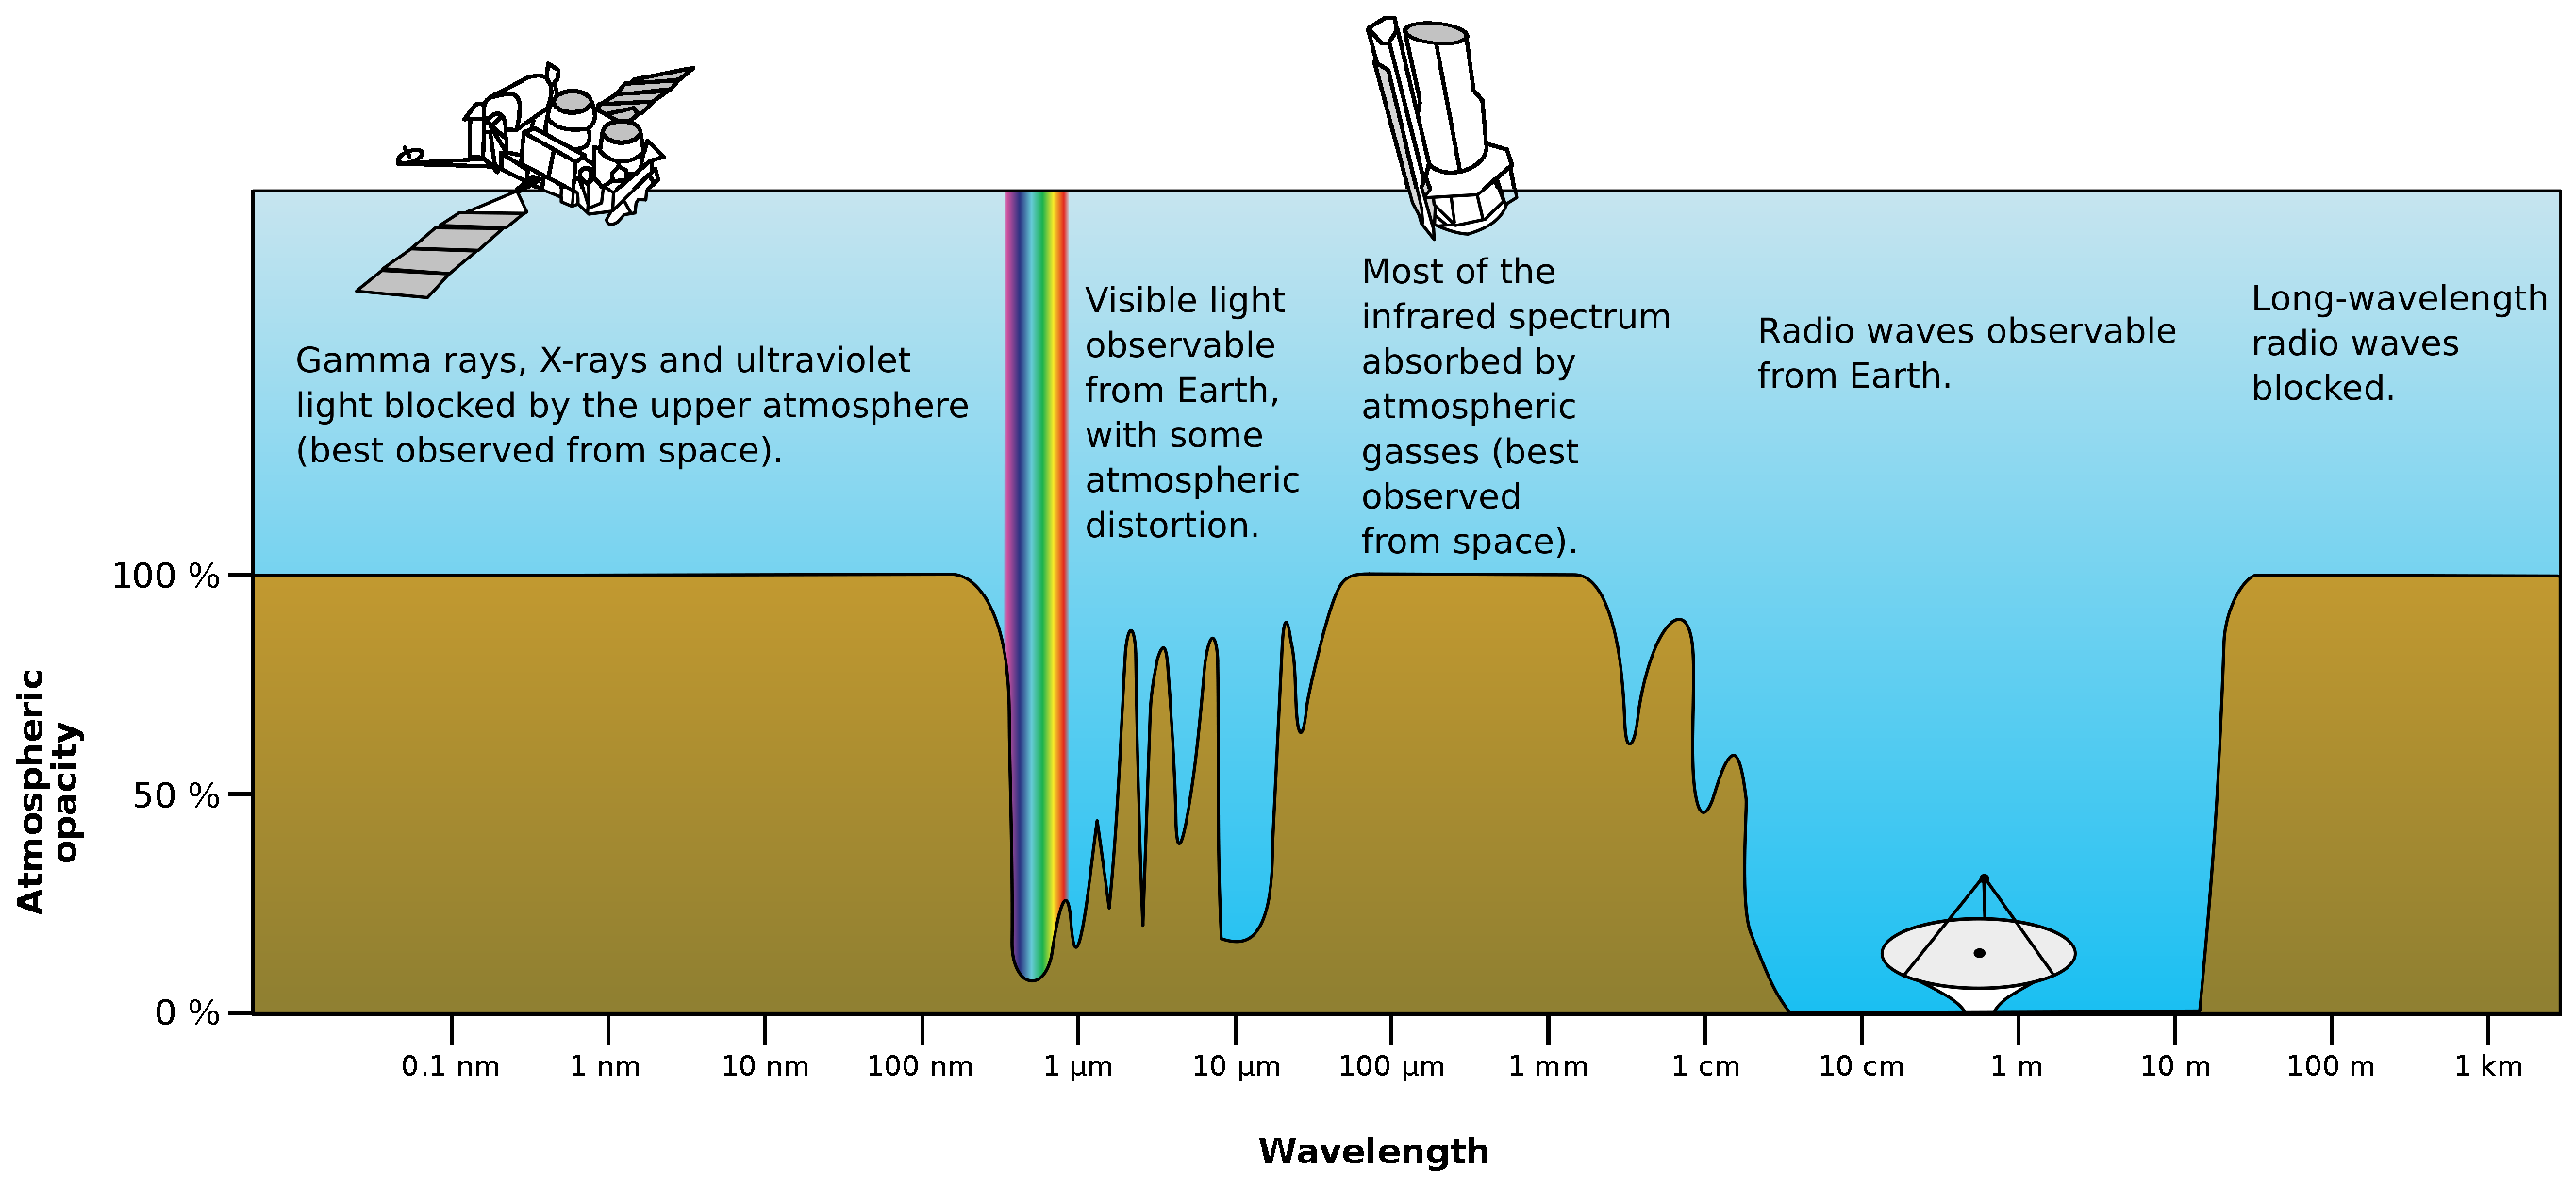
\includegraphics[width=1\linewidth]{Atmospheric_electromagnetic_opacity}
	\end{center}
	\caption{Permeazione dei segnali elettromagnetici nell'atmosfera}
	\label{fig:atm_em_op}
\end{figure}
I segnali elettromagnetici sono fondamentali per lo studio dei corpi celesti.
Tuttavia va considerata la permeabilit\`a dell'atmosfera terrestre rispetto ai
segnali che ci arrivano dallo spazio, come illustrato in Figura
\ref{fig:atm_em_op}: come si pu\`o notare, lo studio dei corpi celesti da terra
\`e possibile solo nello spettro visibile (telescopi, con qualche distorsione)
oppure nello spettro delle frequenze radio (radiotelescopi). Per altre lunghezze
d'onda, \`e necessario studiare questi segnali direttamente dallo spazio con
l'ausilio di satelliti. Il nostro interesse nei capitoli seguenti sar\`a
unicamente incentrato sui segnali radio.

\section{ADC: Analog--to--Digital Conversion}
Per interpretare i segnali del mondo che ci circonda, possiamo sfruttare la
velocit\`a di calcolo di un elboratore; tuttavia per poterlo usare, bisogna
essere in grado di rappresentare le informazioni che riceviamo in modo che
l'elaboratore sia in grado di capirle. Per questo motivo dobbiamo trovare un
modo di trasformare un segnale \emph{analogico} in un segnale \emph{digitale}.

\subsection{Segnali analogici, segnali digitali}
Come abbiamo visto nella definzione \ref{def:signal}, i segnali hanno due
componenti: il tempo e il valore assunto dalla grandezza fisica che osserviamo.
Queste due componenti possono assumere un qualunque valore reale, cio\`e il
segnale ha \emph{tempo continuo} e \emph{valori continui}. Tuttavia, in questo
modo il segnale non pu\`o essere rappresentato da un elaboratore, in quanto un
elaboratore pu\`o contenere solamente quantit\`a finite, mentre le componenti
del segnale sono quantit\`a infinite. Per questo motivo bisogna cercare di far
rientrare il segnale in un range di valori finiti e renderlo cos\`i
rappresentabile da un calcolatore.

Per rendere finita la misurazione del tempo, si possono salvare i valori
rilevati ad un intervallo prefissato, ad esempio una volta ogni secondo.
Misurando un segnale per 10 secondi si otterranno cos\`i 10 valori associati ad
ogni secondo. Un segnale di questo tipo ha \emph{tempo discreto}, ma valori
ancora \emph{continui}. Un dispositivo che raccoglie valori con una determinata
frequenza si chiama \emph{campionatore}.

Per rendere i valori finiti, si pu\`o scegliere di utilizzare un certo insieme
di grandezze, ad esempio $1$ e $-1$, e per ogni valore rilevato, associare la
grandezza pi\`u vicina. Quindi se rileviamo i valori $4$, $10$, $-5$ e $-13$,
salviamo il segnale con i valori $1$, $1$, $-1$, $-1$. Cos\`i facendo, il
segnale assume \emph{valori finiti} che sono rappresentabili in un elaboratore,
nell'esempio fatto con l'uso di 1 bit. Un dispositivo che associa ai valori
rilevati il pi\`u vicino valore rappresentabile dall'elaboratore si chiama
\emph{quantizzatore}.

Un segnale che ha tempo \emph{continuo} e valori \emph{continui} si chiama
\emph{segnale analogico}, mentre un segnale con tempo \emph{discreto} e valori
\emph{finiti} si chiama \emph{segnale digitale}.

Come \`e facile intuire, la conversione da analogico a digitale pu\`o introdurre
degli \emph{errori}, cio\`e del \emph{rumore}, in quanto la versione digitale di
un segnale analogico \`e una approssimazione. Fortunatamente \`e possibile
valutare questo margine di errore e ridurlo a seconda delle necessit\`a sia
aumentando il numero di bit usati per rappresentare i valori nel tempo, sia
aumentando il numero di rilevazioni effettuate nello spazio temporale di
osservazione.

\subsection{Teorema del Campionamento}
Quando si effettua il campionamento di un segnale $f(t)$, si sceglie un periodo
$\tau$ e si fanno $n$ misurazioni nel tempo, ottenendo quindi un segnale di
tipo $f(n\tau)$. Come possiamo assicurarci che da $f(n\tau)$ sia possibile
ricostruire il segnale originale $f(t)$?
Il teorema del campionamento fornisce una risposta definendo un limite basato
sulla frequenza massima del segnale:
\begin{theorem} \label{the:nyquist}
	Un segnale $f(t)$ con frequenza massima $\nu_m$ pu\`o essere ricostruito dal
	segnale campionato $s(n\tau)$ con frequenza $\nu_s = \frac{1}{\tau}$ se
	$\nu_s > 2\nu_m$
\end{theorem}
Cio\`e la frequenza di campionamento deve essere doppia rispetto alla frequenza
massima presente nel segnale.\footnote{Per una dimostrazione del teorema del
campionamento, fare riferimento a \cite{MDFT07}} Nel caso in cui un segnale venga campionato con
frequenza di campionamento $\nu_s < 2\nu_m$, si verifica un fenomeno di
\emph{aliasing}, cio\`e le componenti a frequenza maggiore di $\frac{\nu_s}{2}$
verranno ricostruite come se avessero un'altra frequenza compresa tra $0$ e
$\frac{\nu_s}{2}$; a questo modo l'intero segnale verrebbe compromesso e sarebbe
impossibile recuperare il segnale originario. Per evitare che ci\`o accada si
applica un filtro al segnale che deve essere campionato per eliminare tutte le
frequenze maggiori di $\frac{\nu_s}{2}$, evitando che frequenze non di nostro
interesse possano interferire con le frequenze che andremo ad elaborare.

\section{La Trasformata Discreta di Fourier}
\subsection{Introduzione alla Trasformata di Fourier}
Jean Baptiste Joseph Fourier, vissuto a cavallo tra il XVIII e IX secolo, era
un matematico francese che, presentando i suoi  studi sulla propagazione del
calore, affermava che qualunque segnale periodico continuo potesse essere
rappresentato come somme pesate di sinusoidi. Questa teoria fu molto osteggiata
da Joseph Louis Lagrange, il quale sosteneva che per segnali che contenessero
angoli, come ad esempio le onde quadre, e per questo il lavoro di Fourier non fu
pubblicato per 15 anni, fino alla morte dello stesso Lagrange. In realt\`a
l'approccio di Fourier non era sbagliato, ma anche l'obiezione di Lagrange \`e
valida: se da un lato \`e vero che un segnale con angoli non potesse essere
rappresentato come somme di sinusoidi, si riesce ad ottenere una approsimazione
cos\`i accurata del segnale da avere una differenza energetica pari a zero.
Questo fenomeno \`e conosciuto come \emph{Fenomeno di Gibbs}\footnote{cfr.
\cite{TSEGDSP97}, capitolo 11}

\subsection{Tipi di Trasformate di Fourier}
Esistono quattro tipi di segnali possibili, ognuno con la sua trasformata di
Fourier. Un segnale pu\`o essere periodico o aperiodico, continuo o discreto. Ne
conseguono i quattro tipi di trasformate:
\begin{itemize}
	\item \textbf{Aperiodico - Continuo}: Il segnale non ha \`e periodico ed
		assume infiniti valori. Per analizzarlo si utilizza la \emph{Trasformata
		di Fourier}.
	\item \textbf{Periodico - Continuo}: Il segnale assume infiniti valori che
		si ripetono con un certo periodo. In questo caso si usa la \emph{Serie
		di Fourier}.
	\item \textbf{Aperiodico - Discreto}: Il segnale non ha periodo e assume
		solo un numero finito di valori. In questo caso si utilizza la
		\emph{Trasformata di Fourier a tempo discreto}.
	\item \textbf{Periodico - Discreto}: Il segnale assume un numero finito di
		valori che si ripetono con un dato periodo. La trasformata utilizzata
		\`e la \emph{Trasformata discreta di Fourier}.
\end{itemize}
Ogni segnale usato per queste trasformate deve essere infinito; nel caso in cui
ci fosse un segnale discreto con un numero di punti finito, come succede quando
abbiamo un segnale rappresentato all'interno di un elaboratore, si pu\`o
immaginare questo segnale come se fosse infinito. Se si immagina che prima e
dopo del segnale in nostro possesso il segnale abbia un valore pari a 0, si
user\`a la trasformata di Fourier a tempo discreto, altrimenti se si immagina il
segnale infinito come una ripetizione dei dati in nostro possesso, si utlizza la
trasformata discreta di Fourier. Purtroppo, un qualunque segnale aperiodico ha
infinite componenti sinusoidali, quindi la trasformata di Fourier a tempo
discreto non \`e utilizzabile con un elaboratore, lasciando unicamente la
trasformata discreta di Fourier a nostra disposizione.

Ognuna delle quattro trasformate pu\`o essere eseguita nella sua forma
complessa, dove un insieme di numeri complessi vengono trasformati in un'altro
insieme di numeri complessi, oppure nella forma reale, dove un insieme di numeri
reali vengono trasformati in due insiemi di numeri reali. La forma complessa
di una trasformata \`e molto pi\`u difficile da comprendere, perci\`o verr\`a
esposta unicamente la forma reale della trasformata.

\subsection{Analisi e Sintesi}
Quando applichiamo la trasformata di Fourier, non facciamo altro che passare tra
due rappresentazioni diverse dello stesso segnale: il segnale originario \`e nel
dominio del tempo, mentre il segnale trasformato \`e nel dominio delle
frequenze. Esiste anche la trasformata inversa, che permette di passare dal
dominio della frequenza al dominio del tempo.
L'operazione che trasforma un segnale nel dominio del tempo ad uno nel dominio
delle frequenze si chiama \emph{analisi}, \emph{decomposizione} o semplicemente
{trasformata DFT}, mentre l'operazione inversa si chiama \emph{sintesi} o
{trasformata inversa}. Entrambe le operazioni possono essere espresse come
algoritmi ed utilizzate da elaboratori.

Quando rappresentiamo un segnale in un elaboratore, avremo un vettore,
\texttt{x[]}, contente le ampiezze del segnale nei vari intervalli di tempo. Se
al momento del campionamento abbiamo scelto di misurare $N$ campioni, avremo ora
un vettore di $N$ elementi che vanno da 0 a $N$. Di solito per facilitare la
computazione tramite elaboratore $N$ viene scelto tra le potenze di 2, come
vedremo nel paragrafo \ref{fft}. La controparte di questo segnale \`e suddivisa
in due parti, \texttt{ReX[]} contenente i valori per le ampiezze dei coseni
presenti nel segnale, e \texttt{ImX[]} contenente i valori per le ampiezze dei
seni presenti nel segnale.\footnote{Le notazioni \texttt{ReX[]} e
\texttt{ImX[]} significano, rispettivamente, ``parte reale di X'' e ``parte
immaginaria di X''. Questi nomi provengono dalla versione complessa della
trasformata, ma in questo caso i due vettori vanno considerati semplicemente
come ampiezze dei coseni e dei seni presenti nel segnale.} I due vettori
\texttt{ReX[]} e \texttt{ImX[]} contengono $N/2 + 1$ valori ciascuno, partendo
da 0 e arrivando a $N/2$.

\subsection{Funzioni base della DFT}
Quando effettuiamo la DFT di un segnale, otteniamo due vettori che rappresentano
l'ampiezza delle funzioni di base della DFT. Queste funzioni base sono le
funzioni coseno e seno di diversa frequenza e ampiezza unitaria che fanno parte
del segnale. Quindi avremo che:
\[
\begin{array}{c}
c_k[i] = \cos\left(\frac{2\pi ki}{N}\right)\\[0.5em]
s_k[i] = \sin\left(\frac{2\pi ki}{N}\right)\\[0.5em]
i = 0\dots N-1, \quad k = 0 \dots N/2
\end{array}
\]
Al variare di $k$, varia la frequenza della sinusoide negli $N$ punti: per $k =
0$ avremo $0$ cicli negli $N$ punti, per $k=1$ avremo 1 ciclo, per $k=2$ ci
saranno due cicli e cos\`i via. Ad ogni $c_k$ ed $s_k$, si associano le relative
ampiezze \texttt{ReX[k]} ed \texttt{ImX[k]}.

Tre aspetti importanti vanno notati:
\begin{itemize}
	\item $\boldsymbol{c_0}$ ha valore 1 per tutti i punti $N$:
		$\cos\left(\frac{2\pi 0i}{N}\right) = \cos(0) = 1, \quad \forall i \in
		(0 \dots N-1)$
	\item $\boldsymbol{s_0}$ ha valore 0 in tutti i punti $N$:
		$\sin\left(\frac{2\pi 0i}{N}\right) = \sin(0) = 0, \quad \forall i \in
		(0 \dots N-1)$
	\item $\boldsymbol{s_{N/2}}$ ha valore 0 in tutti i punti $N$:
		$\sin\left(\frac{2\pi N/2i}{N}\right) = \sin(\pi i) = 0, \quad \forall i \in
		(0 \dots N-1)$
\end{itemize}

In particolare si nota che i valori \texttt{ImX[0]} e \texttt{ImX[N/2]} non
influiscono in nessun modo, quindi vengono generalmente impostati a 0. 

\subsection{DFT inversa}
Per ottenere il segnale originario dal segnale nel dominio delle frequenze basta
effettuare la somma dei coseni e dei seni pesati:
\[
x[i] = \sum_{k=0}^{N/2} Re\bar{X}[k] \cos\left(\frac{2\pi ki}{N}\right) +
\sum_{k=0}^{N/2} Im\bar{X}[k] \sin\left(\frac{2\pi ki}{N}\right)
\]
Nell'equazione si usano le versioni normalizzate dei vettori:
\texttt{ReX[]} e \texttt{ImX[]}:
\[
\begin{array}{l}
	Re\bar{X}[k] = \frac{ReX[k]}{N/2}\\[0.5em]
	Im\bar{X}[k] = -\frac{ImX[k]}{N/2}
\end{array}
\]
Ci sono due casi speciali:
\[
\begin{array}{l l}
	Re\bar{X}[0] & = \frac{ReX[0]}{N} \\[0.5em]
	Re\bar{X}[N/2] & = \frac{ReX[N/2]}{N}
\end{array}
\]
Questa normalizzazione viene introdotta perch\'e il dominio delle frequenze \`e
definito come densit\`a spettrale, cio\`e le frequenze sono divise in bande e
ogni valore \texttt{ReX[]} e \texttt{ImX[]} rappresenta la quantit\`a di segnale
(ampiezza) presente per ogni unit\`a dell'ampiezza di banda: ad esempio il
valore \texttt{ReX[1]} rappresenta l'ampiezza del segnale nella banda 1, che
corrisponde all'intervallo $0,5\dots1,5$, \texttt{ReX[2]} rappresenza l'ampiezza
del segnale nella banda 2 ($1,5\dots2,5$) e cos\`i via. Ci sono $N/2+1$ bande,
quindi ogni banda \`e larga $\frac{1}{N/2} = \frac{2}{N}$, tranne la prima e
l'ultima: la banda 0 ($0\dots 0.5$) e la banda $N/2$ ($N/2-0,5\dots N/2$) sono
larghe esattamente la met\`a, $\frac{1}{N}$.

\subsection{FFT: Fast Fourier Transform}
\label{fft}
Taken from \cite{bertoni}

\chapter{Progettazione e architettura}
\label{outline}
Nel momento della progettazione, sono stati prefissati alcuni punti importanti:
il programma avrebbe dovuto essere veloce, modulare e parametrizzabile sulle
caratteristiche pi\`u rilevanti dei segnali. L'utilizzo del C++ come linguaggio di
sviluppo ha portato alla scelta di scrivere preferibilmente codice orientato
agli oggetti e di sfruttare al massimo gli strumenti offerti dalla libreria
boost\footnote{\url{http://www.boost.org/}}, praticamente uno standard per qualunque programma C++ di una certa
complessit\`a.
\section{Obiettivi}
Il funzionamento desiderato per l'applicazione \`e piuttosto semplice: il
programma legge dei dati da una sorgente, li trasforma con una \ac{FFT} ed
eventualmente applica qualche filtro, infine scrive l'output su una qualche
destinazione. Un importante obiettivo \`e che la manipolazione dei segnali
avvenga in real---time, cio\`e che le operazioni vengano calcolate abbastanza
velocemente da riuscire ad elaborare i dati man mano che arrivano dalla
sorgente.

Uno degli utilizzi principali ipotizzati per lo spettrometro \`e l'elaborazione
di dati per il progetto \ac{seti}. In questo caso, i dati vengono recuperati da
una speciale scheda di acquisizione dedicata\footnote{L'hardware necessario a
sviluppare questo aspetto dell'applicazione non era disponibile, perci\`o
    l'implementazione dell'acquisizione di dati \ac{seti} \`e stata lasciata
    come possibile sviluppo futuro. cfr. \ref{seti}}.
Le caratteristiche fondamentali della \ac{FFT} sono una lunghezza del segnale
piuttosto importante (circa $2^{23}$), un basso numero di integrazioni e la
possibilit\`a di ricevere i dati sporadicamente, cio\`e il data rate pu\`o
essere mantenuto basso.

Un'altro utilizzo \`e l'analisi di space debris(?) dove la sorgente di dati sono
dei pacchetti UDP e la \ac{FFT} \`e caratterizzata da segnali di lunghezza contenuta
(circa $2^{15}$) con molte integrazioni (circa $100000$). In questo caso \`e
importante riuscire a mantenere il data rate alto, quindi l'elaborazione deve
essere il pi\`u veloce possibile.

\section{Gerarchia di classi}
Per raggiungere gli obiettivi prefissati, sono necessarie alcune classi per
astrarre alcuni concetti. In particolare ci sono tre componenti fondamentali:
\begin{itemize}
\item Una sorgente da cui prendere dati
\item Filtri o trasformazioni da applicare al segnale
\item Una destinazione su cui scrivere l'output
\end{itemize}
Per questo motivo ci sono tre classi astratte che rappresentano questi tre
concetti: \\
\texttt{SourceFilter}, \texttt{ProcessFilter} e \texttt{SinkFilter}.
\subsection{SourceFilter}
Una sorgente ha un unico metodo assolutamente necessario che serve a leggere i
dati. Una sottoclasse di \texttt{SourceFilter}, ad esempio, \`e il server UDP
(\texttt{udp\_sock}), che pu\`o essere usata da qualunque codice generico che
faccia riferimento unicamente all'interfaccia astratta. Se si creasse un'altra
sottoclasse di \texttt{SourceFilter} e la si sostituisse a \texttt{udp\_sock} si
otterrebbero i dati da un'altra fonte senza dover cambiare una riga di codice al
di fuori della inizializzazione.
\subsection{ProcessFilter}
Un \texttt{ProcessFilter} rappresenta una qualunque elaborazione intermedia del
segnale, sia essa una trasformata di Fourier o un filtro passa---basso o una
qualunque altra manipolazione. Siccome in questa fase si prende un segnale e lo
si manipola in qualche maniera, l'interfaccia richiede un metodo
\texttt{transform} che abbia in input i dati da elaborare e scriva su un vettore
di output specificato. I filtri sono per natura concatenabili, quindi per
gestire questa coda serve una classe \texttt{FilterChain} che si occupi di
passare l'elaborazione attraverso una coda di filtri precedentemente
selezionati.
\subsection{SinkFilter}
Le destinazioni hanno bisogno di un unico metodo di interfaccia: \texttt{write}.
In modo simile al \texttt{SourceFilter}, una qualunque implementazione della
classe astratta \texttt{SinkFilter} pu\`o essere intercambiata con un'altra
senza dover apportare modifiche al codice, permettendo di scegliere il
dispositivo di memorizzazione pi\`u adeguato agli scopi perseguiti.
\subsection{Contenitori di dati}
Sono state progettate alcune classi al fine di astrarre i dati e assicurarne la corretta sincronizzazione.
\subsubsection{SrcType}
\texttt{SrcType} \`e una struttura con un costruttore, un destruttore ed un operatore di assegnamento. Tra i membri di questa struttura c'\`e una mutex per eseguire operazioni in mutua esclusione, ove necessario. Questa struttura \`e un wrapper di un puntatore, ideale per essere usata all'interno di un circular buffer.
\subsubsection{FFTBuf}
La classe \texttt{FFTBuf} \`e un vettore su cui vanno scritti i risultati di una o pi\`u trasformazioni di Fourier. Al momento della costruzione, si indica la lunghezza del segnale da salvare e il numero di integrazioni che si prevede di fare; a questa maniera \`e possibile assegnare questo buffer a tanti thread quante dovranno essere le integrazioni da fare. La classe offre strumenti anche per tener traccia di quante integrazioni sono già state effettuate e sapere cos\`i se il buffer \`e pronto per essere scritto su output.
\subsubsection{List}
La classe \texttt{List} \`e un semplice wrapper attorno ad una lista della libreria standard. Questa classe assicura un comportamento corretto in ambienti multithreading e aggiunge alcuni metodi per semplificare la coordinazione con gli altri thread.
\subsection{Wrapper di librerie}
La classe \texttt{IPP} esiste solo per fornire un wrapper C++ alle librerie \ac{ipp}, scritte in C. Tramite overloading \`e stato possibile utilizzare lo stesso nome per funzioni che operano su tipi di dati differenti, lasciando al compilatore il compito di invocare la funzione specifica pi\`u adeguata.

\chapter{Sviluppo del progetto}
\label{sw_devel}

Durante lo sviluppo del progetto si ha fatto uso di librerie e strumenti
software per semplificare il pi\`u possibile il lavoro da svolgere ed ottenere
il massimo delle prestazioni possibili. 

\section{Librerie}
L'utilizzo delle giuste librerie permette di sviluppare pi\`u velocemente i
propri progetti, ottenere prestazioni spesso migliori rispetto ad una soluzione
sviluppata in proprio e sicuramente avere pi\`u certezze riguardo al corretto
funzionamento delle parti attenenti alla libreria.

\subsection{Boost}
Le librerie Boost\footnote{\url{http://www.boost.org/}} sono molto usate nella
programmazione in \CC perch\'e implementano moltissime funzioni di comune
utilizzo fornendo una interfaccia molto semplice. L'ottima qualit\`a di queste
librerie \`e confermato dal fatto che spesso alcune sue componenti vengono
integrate nello standard \CC. Queste librerie sono basate sulla versione ANSI
del \CC, rendendole compatibili con qualunque compilatore che implementi gli
standard ANSI.In questo progetto vengono utilizzate principalmente per
semplificare la lettura di argomenti da linea di comando, la lettura/scrittura
di files, le comunicazioni di rete e il multi-threading.

\subsection{\ac{ipp}}
Le Integrated Performance
Primitives\footnote{\url{http://software.intel.com/en-us/intel-ipp/}} sono delle
librerie che implementano un insieme molto completo di funzioni e algoritmi
relativi al processamento di segnali e crittografia. In particolare implementano
funzioni utili al processamento di segnali audio (filtri, codifiche audio,
compressione dei dati, ecc.), funzioni per il processamento di immagini
(trasformazioni, codifica video, ecc.), funzioni per calcoli su matrice e
funzioni crittografiche (crittografia simmetrica, asimmetrica, funzioni hash,
ecc.).  Il vantaggio delle IPP \`e che offrono un ampio spettro di funzioni che
coprono praticamente tutte le necessit\`a nel processamento dei segnali, oltre
ad essere ottimizzate per processori Intel. Inoltre sono state scritte in modo
da essere naturalmente utilizzabili in ambienti multi-threaded, sfruttando tutte
le potenzialit\`a di processori multicore o processori multipli. Tutti questi
fattori hanno concorso nell'adozione di questa libreria al posto di altre
librerie concorrenti. Questa libreria \`e l'unico componente non Open Source
utilizzato nell'intero progetto, anche se il suo utilizzo \`e gratuito per usi
accademici. Le librerie alternative potrebbero essere comparate per verificare
l'effettiva qualit\`a a livello di prestazioni\footnote{cfr. paragrafo
\ref{altlib}}.

\subsubsection{Multithreading e prestazioni nelle \ac{ipp}}
Le \ac{ipp} sono state sviluppate con l'intenzione di sfruttare a pieno le
istruzioni \ac{SIMD} e \ac{SSE} presenti nei moderni processori. Queste
istruzioni permettono di effettuare operazioni su vettori in parallelo,
guadagnando grandi vantaggi prestazionali in alcuni tipi di operazioni, tra cui
anche i calcoli necessari per l'elaborazione di segnali. Siccome diversi
processori supportano diversi tipi di istruzioni, possono esistere diverse
implementazioni di alcune funzione in base al tipo di istruzioni supportate. Per
selezionare automaticamente la funzione corretta, le \ac{ipp} dispongono di un
dispatcher che, durante l'inizializzazione a run-time, individuano le capacit\`a
del processore e quindi la categoria di libreria da utilizzare. Questo permette
di usare trasparentemente le funzioni di libreria sfruttando sempre
l'implementazione pi\`u efficiente per il processore utilizzato.

Alcune funzioni di base della libreria sfruttano il threading per migliorare le
proprie prestazioni, in particolare sfruttando le librerie OpenMP sviluppate da
Intel. Quando si utilizza la versione multi-threaded della libreria, i thread
vengono automaticamente inizializzati al numero di processori e core presenti: a
questo modo la libreria avvier\`a al massimo tanti thread quante sono le unit\`a
di calcolo presenti nel sistema, evitando di sovracaricare il sistema e
ottenendo cos\`i la migliore prestazione possibile dal sistema in uso. Sono
presenti anche due funzioni, \texttt{ippSetNumThreads()} e
\texttt{ippGetNumThreads()}, che permettono di manipolare il numero di threads
utilizzati dalla libreria. Il numero di thread non sar\`a mai maggiore rispetto
al numero di unit\`a di calcolo del sistema, anche se impostati manualmente ad
un valore maggiore.

Tutte le funzioni IPP sono thread-safe, cio\`e possono essere usate da diversi
thread di esecuzione contemporaneamente senza che questo implichi un qualunque
malfunzionamento.\footnote{Per approfondimenti, cfr.
\url{http://software.intel.com/en-us/articles/threading-and-intel-integrated-performance-primitives/}}


\section{Codice pre-esistente}
Parte del codice del progetto \`e stato prelevato dal software sviluppato in
fase di tirocinio, sempre presso l'Istituto di Radioastronomia di Medicina.
Questo codice ha permesso di ridurre notevolmente il tempo dedicato allo
sviluppo del calcolo della \ac{FFT} lasciando maggior tempo per una corretta
implementazione delle altre parti. Questo codice \`e stato adattato per
funzionare in un contesto multi-threaded e per accettare input da diverse fonti.

\section{Gestione di problemi comuni}
\subsection{Selezione del tipo di dato}
Per rendere il programma il pi\`u versatile possibile, non si poteva legare il
suo funzionamento ad un unico tipo di dati. Siccome le \ac{ipp} includono
funzioni per diversi tipi di dati, il programma \`e stato sviluppato in modo da
riuscire a selezionare il giusto tipo di funzione a seconda del tipo di dato in
input e in output. L'implementazione attuale permette di selezionare il tipo di
dato impostando delle costanti e ricompilando il codice, un possibile
miglioramento potrebbe essere la selezione dinamica senza bisogno di
ricompilazione del tipo di dato, cui parleremo nel paragrafo \ref{dyn_dtype}.

\subsubsection{Dal numero di bit al tipo di variabile}
Il primo passo da compiere per poter lavorare sul tipo di dato desiderato \`e
associare al numero di bit selezionati nella costante il corretto tipo di dato.
Il listato \ref{lst:consts_def} illustra il metodo di selezione dei numeri di bit e
la definizione delle costanti contenenti i tipi di dato corretti. Come si pu\`o
osservare, si usano i template per ottenere il risultato che vogliamo e con
delle \texttt{typedef} definiamo dei nuovi tipi corrispondenti alle dimensioni
richieste. Parte del codice di \texttt{typer} \`e riportato nel listato
\ref{lst:typer}. Si pu\`o osservare come molto semplicemente al variare dei due
parametri del template, si definisce un tipo denominato \texttt{type}
corrispondente alle caratteristiche richieste.

\lstinputlisting[firstline=25,lastline=34,float,caption=Definizione di costanti
per la selezione del tipo di
dato,label=lst:consts_def,basicstyle=\tiny]{../src/main.cc}

\lstinputlisting[firstline=4,lastline=21,float,caption=La magia dietro
\texttt{typer},label=lst:typer,basicstyle=\small]{../src/type.hpp}

\subsubsection{Gestione della memoria}
La libreria \ac{ipp} fornisce alcune funzioni per allocare memoria
allineata\footnote{TBA} ed effetuare altre operazioni di basso livello. Siccome
la libreria \`e scritta in C, ogni tipo di dato ha una funzione diversa, quindi
per poter scrivere codice generico che funzioni con qualunque tipo di dato \`e
stato necessario creare un'interfaccia \CC che richiami automaticamente le
funzioni corrette. Il metodo adottato (listato \ref{lst:malloc}) prevede che la
funzione generica di interfaccia prenda due argomenti invece di uno solo: il
primo argomento \`e un puntatore al vettore per cui si sta allocando la memoria
ed il secondo argomento \`e la lunghezza di questo vettore. Il primo argomento
in realt\`a non viene utilizzato, ma con la tecnica dell'\texttt{overloading}
permette di selezionare la funzione corretta.

\lstinputlisting[firstline=108,lastline=130,float,caption=Alcune implementazioni
della funzione
\texttt{IPP::malloc},label=lst:malloc,basicstyle=\small]{../src/ipp.cc}

\subsubsection{Buffer di dati}
Per le classi e strutture contenente i dati \`e stata scelta una strategia
diversa: siccome non \`e necessario chiamare funzioni di libreria, ma i metodi
sono generici ed indipendenti dal tipo di dato su cui si opera, sono stati
adottati i template come soluzione generica. Come si pu\`o vedere nella
definizione della struttura \texttt{SrcType} (listato \ref{lst:srctype}), i
membri della struttura sono assolutamente neutri rispetto al tipo di dato
utilizzato.

\lstinputlisting[firstline=227,lastline=236,float,caption=Dichiarazione della
struttura \texttt{SrcType},label=lst:srctype]{../src/fft_buf.hpp}

\subsection{Client UDP come SourceFilter}
Nel paragrafo \ref{sourcefilter} abbiamo spiegato come in fase di progettazione
si sia pensato ad una interfaccia generica per leggere i dati da una fonte
esterna; il listato \ref{lst:sourcefilter} mostra l'implementazione di questa
interfaccia.
\lstinputlisting[firstline=4,lastline=10,float,caption=Dichiarazione
dell'interfaccia
\texttt{SourceFilter},label=lst:sourcefilter]{../src/filter/source.hpp}

Per implementare questa interfaccia \`e sufficiente ereditare dalla classe
virtuale \texttt{SourceFilter} ed implementare il metodo \texttt{read()}.
Vediamo ad esempio la dichiarazione della classe \texttt{udp\_sock}, presentata
nel listato \ref{lst:udp_sock}: si pu\`o notare che vengono definite due
funzioni read, una delle quali corrisponde a quella dichiarata nella classe
virtuale \texttt{SourceFilter}. L'implementazione della \texttt{read()}
virtuale, presentata nel listato \ref{lst:udp_read}, non fa altro che convertire
il puntatore a void in un puntatore del tipo specificato dal template. Questo
permette di usare la classe \texttt{udp\_sock} con qualunque tipo di dato.

\lstinputlisting[firstline=25,lastline=41,caption=Dichiarazione della classe
\texttt{udp\_sock},float,label=lst:udp_sock,basicstyle=\small]{../src/server.hpp}

\lstinputlisting[firstline=183,lastline=186,caption=Implementazione della
\texttt{read()} virtuale,float,label=lst:udp_read]{../src/server.hpp}

\subsection{Gestione del threading}
Quando si introduce il threading in una applicazione, ci sono delle situazioni
che vanno prese in considerazione: avere diversi thread pu\`o portare problemi
normalmente assenti e non facilmente identificabili. Inoltre alcuni problemi
legati al threading possono essere difficili da riprodurre perch\'e  dipendono
dalla schedulazione dei thread da parte del sistema operativo, quindi sono al di
fuori dal controllo del programmatore. Per questo motivo esistono alcune
tecniche di programmazione che permettono di evitare problemi quando thread
diversi devono condividere alcuni dati.

\subsubsection{Mutua esclusione}
\lstinputlisting[firstline=3,lastline=12,float,caption=Variabili della
lista,label=lst:vars]{../src/list.hpp}
Con la mutua esclusione si assicura che quando un thread accede ad una parte di
dati protetta, nessun altro thread pu\`o accedervi contemporaneamente. La mutua
esclusione \`e stata implementata, ad esempio, come wrapper attorno alla
struttura standard \texttt{std::list} per renderla utilizzabile da pi\`u thread
contemporaneamente.

Per rendere la lista thread-safe, servono tre variabili: una contiene la lista
standard, una per la mutex ed una per la condition variable, come mostrato nel
listato \ref{lst:vars}

Una mutex, abbreviazione di \textbf{mut}utal \textbf{ex}clusion, serve appunto
per poter bloccare l'accesso all'oggetto da parte di altri thread e per
rilasciare il blocco quando si ha finito. Le funzioni presenti in
\texttt{std::list} vengono reimplementate sfruttando la mutex per assicurare un
comportamento corretto in caso di multi-threading: troviamo un buon esempio nel
metodo \texttt{empty()} presentato nel listato \ref{lst:empty}.
\lstinputlisting[firstline=24,lastline=28,float,caption=Implementazione di
\texttt{empty()},label=lst:empty]{../src/list.hpp}

La creazione dell'oggetto di tipo \texttt{boost::mutex::scoped\_lock} sospende
l'esecuzione del thread se ci sono gi\`a altri thread che possiedono l'esclusiva
sull'oggetto \texttt{\_mut}, altrimenti acquisisce il diritto di esclusiva
sulla mutex e procede con l'operazione. Nel distruttore dell'oggetto
\texttt{lock} avviene il rilascio della mutex, quindi non appena l'oggetto
finisce fuori contesto --- cio\`e dopo il \texttt{return} --- il distruttore
viene chiamato e la mutex viene liberata, lasciando libero accesso ad altri
threads.

\subsubsection{Wait/notify}
Abbiamo visto nel paragrafo \ref{threadout} come il thread di output si metta in
attesa sulla lista quando questa \`e vuota. Il codice presente nel thread di
output \`e simile a questo:
\begin{lstlisting}
while(list.empty()) {
    list.wait();
}
//Do something
\end{lstlisting}

Questo codice mette in uno stato ``dormiente'' il thread, lasciando il posto
agli altri thread e ottimizzando cos\`i il tempo di scheduling assegnato al
programma: l'alternativa sarebbe fare un ciclo continuo --- detto \emph{busy waiting} --- per verificare la stessa
condizione ripetutamente, ma in questo modo si sprecherebbero tantissime risorse
su un controllo che non cambier\`a risultato prima che avvengano altre cose. Per
monitorare lo stato di questa condizione, si pu\`o utilizzare una
\texttt{boost::condition\_variable}, come mostrato nel listato \ref{lst:cond_wait}.
\lstinputlisting[firstline=50,lastline=53,float,caption=Uso della
\texttt{boost::condition\_variable},label=lst:cond_wait]{../src/list.hpp}
Il codice inizialmente acquisisce un lock esclusivo sulla mutex, poi si mette in
attesa sulla \texttt{condition\_variable} \texttt{\_empty}. A questo punto
il lock viene rilasciato ed il thread si mette in attesa, senza occupare risorse
sul sistema. Per risvegliare questo thread bisogna notificarlo del fatto che la
condizione su cui stava aspettando `e stata modificata, quindi quando si
inserisce un nuovo elemento nella lista bisogna anche notificare il thread di
output che la lista non \`e pi\`u vuota, come illustrato nel listato
\ref{lst:notify}. Il metodo \texttt{notify\_one()} \`e definito come:
\begin{lstlisting}[frame=none]
    void notify_one() { _empty.notify_one(); }
\end{lstlisting}
Utilizza, quindi, la \texttt{condition\_variable} per notificare uno dei thread
in attesa sulla variabile stessa. A questo punto il thread di output si
risveglia, aspetta di poter riacquisire il lock sull'oggetto e continua con
l'esecuzione. A questo punto la condizione \texttt{list.empty()} dovrebbe
essere falsa e il thread pu\`o procedere con il suo lavoro.
\lstinputlisting[firstline=34,lastline=38,float,caption=Notifica di inserimento
di un nuovo elemento in lista,label=lst:notify]{../src/list.hpp}

\subsubsection{Debugging}
Per capire meglio i problemi che possono sorgere osserviamo il codice nel
listato \ref{lst:threrr}:
\begin{lstlisting}[numbers=left,frame=l,float,caption=Codice problematico nel caso
	di pi\`u threads attivi,label=lst:threrr]
if( list.empty() || list.back()->is_src_full() ) {
	FFTBuf<DstIppType> *buffer( new FFTBuf<DstIppType>(siglen, sums) );
	*buffer = IPP::alloc(buffer->cdata(), siglen);
	IPP::zero_mem(buffer->cdata(), siglen);
	list.push_back(buffer);
}
FFTBuf<DstIppType> *work_buffer = list.back();
\end{lstlisting}
questo codice faceva parte del thread principale ed \`e il controllo effettuato
per verificare se \`e necessario creare un nuovo buffer di output o se si pu\`o
assegnare l'ultimo buffer in lista come punto di scrittura della trasformazione
da effettuare, meccanismo descritto nel paragrafo \ref{main_thread}.
\paragraph{Analisi del codice}
Siccome il listato non \`e banale, procediamo ad analizzare passo per passo le
operazioni effettuate:

Nella riga 1, si controlla innanzitutto se la lista di output \`e vuota o se
l'ultimo elemento nella lista \`e stato assegnato tante volte quanto sono il
numero di somme che si vogliono effettuare. Se almeno una delle due condizioni
\`e vera, significa che dobbiamo accodare un nuovo elemento nella lista. La riga
2 crea il puntatore \texttt{buffer} ed inizializza l'oggetto di tipo
\texttt{FFTBuf<DstIppType>} assegnando come parametri la lunghezza del segnale
elaborato (\texttt{siglen}) ed il numero di somme che si intendono fare su quel
buffer (\texttt{sums}). \texttt{FFTBuf} \`e un oggetto che contiene il buffer in
cui viene salvato il segnale una volta applicate le trasformazioni e alcuni
metodi ausiliari. Uno di questi metodi, usato nella riga 1, \`e
\texttt{is\_src\_full()} che restituisce un valore booleano vero se l'istanza
dell'oggetto \`e stata assegnata ad un numero di thread pari al numero di somme
volute, falso altrimenti. Con questo metodo, quindi, si pu\`o sapere se
l'istanza dell'oggetto \`e riutilizzabile per un altro thread o meno. La
costante DstIppType segnala il tipo di dato su cui si opera, in particolare il
numero di bit usati per ogni punto del segnale: avere questa costante permette
di adattare il programma molto velocemente per tipi di dati diversi. Alle righe
3--4 si alloca la memoria per il buffer, utilizzando i metodi delle \ac{ipp} per
fare s\`i che la memoria sia allineata e la si inizializza a zero.  Nella riga 5
si accoda il puntatore al buffer in quanto ora l'inizializzazione \`e
completata. La riga 7 mostra come viene selezionato il buffer su cui lavorare:
grazie al codice precedente si tratter\`a sempre dell'ultimo buffer inserito
nella lista.

\paragraph{Comportamento in ambiente multi-threaded}
Il codice appena descritto funziona perfettamente se non si utilizza il
threading. Tuttavia, durante la fase di test, il programma funzionava il pi\`u
delle volte, ma presto o tardi l'esecuzione terminava con un errore di
\emph{segmentation fault}\footnote{La segmentation fault \`e un errore tipico
    dei programmi C/\CC. Significa che un programma ha tentato di accedere ad
    una zona di memoria non di sua competenza e il sistema operativo non
    concede di farlo per ovvi motivi di sicurezza. Tipicamente questo problema
    avviene quando si legge oltre la fine di un array o si tenta di accedere ad
    un puntatore non allocato o impostato a NULL.}.
Osservando il problema con l'ausilio di un debugger, il problema non risultava
chiaro perch\'e si presentava in punti differenti del codice e sempre in
situazioni in cui non ci si aspetta di avere un puntatore nullo, rendendo
l'investigazione tramite debugger praticamente inutile. Il fatto che il problema
si mostrasse in modo casuale, in momenti diversi e in punti diversi del codice
lasciava intuire che si trattasse di un problema di concorrenza, quindi
riesaminando l'interazione dei vari thread tra di loro si \`e riusciti a scovare
e risolvere la fonte del problema:  come descritto nel paragrafo
\ref{threadout}, il thread di output lavora sulla lista di buffer e quando
finisce di scrivere i dati sull'output, elimina il buffer dalla lista. Se
osserviamo in particolare la riga 1 del listato \ref{lst:threrr}, vediamo che si
chiede prima se la lista \`e vuota e in seguito si accede all'ultimo elemento in
lista. Ma cosa succede se subito dopo l'istruzione \texttt{list.empty()} avviene
un \emph{context switch} e il thread di output riprende l'esecuzione, scrive
l'ultimo buffer presente il lista sull'output e lo elimina? In questo scenario
la successiva chiamata a \texttt{list.back()} ritornerebbe un puntatore nullo e
la chiamata a \texttt{is\_src\_full()} provoca la segmentation fault. Per
evitare che questo avvenga, bisogna richiedere il lock sulla mutex della lista
di buffer di output prima di testare le condizioni, a questo modo mentre si
verifica questa condizione lo stato della lista non pu\`o essere alterato.

\paragraph{Conclusioni e osservazioni}
La soluzione al problema, presentata nei listati \ref{lst:thr_correct} e
\ref{lst:item_needed} \`e stata raggiunta dopo molto tempo perso a ricercare la
fonte di questo problema causato da una non corretta analisi dei comportamenti
in ottica multi-threaded.  Individuare questo genere di errori \`e molto
difficile, mentre commettere questo tipo di errori \`e molto facile: per questo
motivo \`e generalmente consigliabile evitare la concorrenza a meno che non vi
siano chiari vantaggi nell'adottarla; e quando si decide di sfruttare la
concorrenza nel proprio programma, \`e importante considerare tutti gli scenari
possibili nelle interazioni tra i thread soprattutto quando si effettuano
operazione non atomiche\footnote{Una operazione, ad esempio \lstinline$int i =
    5;$ \`e atomica se la sua esecuzione non pu\`o essere interrotta a met\`a: o
        l'operazione \`e ancora da effettuare, oppure \`e completata. In \CC 
        l'operazione di cui sopra viene tradotta in diverse istruzioni macchina
        e quindi pu\`o avvenire un context switch a met\`a dell'operazione. Le
        istruzioni in \CC, quindi, non sono atomiche. Esistono altri linguaggi
        di programmazione, pensati appositamente per la programmazione
        multi-threaded, che garantiscono l'atomicit\`a delle loro istruzioni.}.
\begin{lstlisting}[float,label=lst:thr_correct,caption=Codice funzionante anche
in ambiente multi-threaded]
if(list.item_needed()) {
	FFTBuf<DstIppType> *buffer( new FFTBuf<DstIppType>(siglen, sums) );
	*buffer = IPP::alloc(buffer->cdata(), siglen);
	IPP::zero_mem(buffer->cdata(), siglen);
	list.push_back(buffer);
}
FFTBuf<DstIppType> *work_buffer = list.back();
\end{lstlisting}
\lstinputlisting[firstline=55,lastline=58,float,caption=Implementazione del
metodo \texttt{item\_needed()},label=lst:item_needed]{../src/list.hpp}

\subsection{Memory leak}
Un altro problema molto diffuso nella programmazione in \CC sono i \emph{memory
leak}. Con questo termine si indicano quelle perdite di memoria che avvengono
perch\'e ad allocazione di memoria da una parte, non corrisponde una
deallocazione da un'altra parte del codice. Se un problema di questo genere
esiste e non viene corretto, un programma che rimane attivo per un certo periodo
di tempo incrementa sempre pi\`u il suo utilizzo di memoria, fino a che la
memoria disponibile nel sistema non viene interamente consumata. A questo punto
non solo il programma non pu\`o pi\`u funzionare, ma anche gli altri programmi
presenti sul sistema possono riscontrare problemi per la mancanza di memoria da
allocare; in alcuni casi il sistema potrebbe diventare addirittura
inutilizzabile e potebbe diventare necessario un riavvio del sistema. Purtroppo,
se la perdita di memoria \`e sufficientemente piccola, \`e facile che un
problema di questo tipo possa sfuggire in fase di test e creare problemi solo
dopo un lungo utilizzo in fase di produzione. Per questo motivo esistono dei
tool, come ad esempio la suite di
Valgrind\footnote{\url{http://www.valgrind.org/}}, che aiutano
nell'individuazione di questi problemi. Durante lo sviluppo del progetto \`e
stato incontrato un errore di questo tipo nell'implementazione del buffer per i
dati di output.

\subsubsection{Implementazione originaria}
La classe \texttt{FFTBuf} contiene un buffer e qualche metodo per gestire
l'accesso al buffer stesso. Nella sua prima versione il codice per
inizializzarlo era il seguente:
\begin{lstlisting}[caption=Inizializzazione di un FFTBuf (vecchia
versione),label=lst:old_fftbuf]
FFTBuf<DstIppType> *buffer( new FFTBuf<DstIppType>(siglen, sums) );
*buffer = IPP::alloc(buffer->cdata(), siglen);
IPP::zero_mem(buffer->cdata(), siglen);
\end{lstlisting}
Come si pu\`o vedere, l'allocazione della memoria veniva effettuata manualmente
dopo l'inizializzazione dell'oggetto, mentre non era presente alcuna
deallocazione della memoria. Per risolvere questo problema ci sono due strade
possibili: o si aggiunge una deallocazione della memoria dopo che i dati sono
stati scritti su output, o si sposta il meccanismo di allocazione/deallocazione
all'interno del costruttore/distruttore della classe. Per rendere l'utilizzo di
\texttt{FFTBuf} pi\`u trasparente ed evitare che il problema si ripeta se questa
classe dovesse essere riutilizzata da qualche altra parte, la scelta \`e
ricaduta sulla seconda soluzione.

\subsubsection{Implementazione corretta}
La nuova versione dell'allocazione di  memoria per il buffer interno a
\texttt{FFTBuf} \`e la seguente:
\begin{lstlisting}
template<class T> FFTBuf<T>::FFTBuf(long int siglen) : _dst(NULL),
    _siglen(siglen), _expected_sums(1), _processed_sums(0),
    _assigned_sources(0), _written(false)
{
    _dst = IPP::alloc(_dst, siglen);
    IPP::zero_mem(_dst, siglen);
}

template<class T> FFTBuf<T>::FFTBuf(long int siglen, int sums) :
    _dst(NULL), _siglen(siglen), _expected_sums(sums),
    _processed_sums(0), _assigned_sources(0), _written(false)
{
    _dst = IPP::alloc(_dst, siglen);
    IPP::zero_mem(_dst, siglen);
}

template<class T> FFTBuf<T>::~FFTBuf()
{
    notify_all();
    IPP::free(_dst);
    _dst = NULL;
}
\end{lstlisting}
Ora l'allocazione \`e legata alla creazione di un nuovo oggetto di tipo
\texttt{FFTBuf} e la deallocazione viene effettuata automaticamente quando
l'oggetto viene distrutto: a questo modo si ha la certezza che tutti i buffer
creati vengono distrutti correttamente e che non ci sar\`a perdita di memoria.
Dopo questa modifica, il programma \`e passato da pochi minuti di operativit\`a
con consumo di memoria sempre crescente a un consumo di memoria stabile e
conseguente stabilit\`a del programma stesso.

\section{Programmi di supporto}
Allo scopo di testare l'applicazione e verificarne il funzionamento, sono stati
sviluppati alcuni programmi di supporto. Trattandosi di programmi in cui le
prestazioni non sono essenziali, il linguaggio di programmazione utilizzato \`e
Python per favorire uno sviluppo pi\`u rapido.
\subsection{Server UDP}
Uno dei programmi sviluppati serve ad inviare dei dati nel formato corretto
tramite il protocollo UDP. Siccome l'ordinamento \`e importante,
anche se non \`e grave l'eventuale perdita di alcuni pacchetti, all'inizio di
ogni pacchetto UDP compare un contatore progressivo lungo 4 byte. Il client
controlla questo contatore e se il numero non \`e in progressione con il
pacchetto precedente, sa quanti pacchetti ha perso e svuota i buffer
eventualmente pieni per ricominciare ad elaborare i dati a partire dal nuovo
pacchetto ricevuto. Questa operazione viene svolta per evitare di elaborare dati
incompleti che potrebbero compromettere i risultati. Il server in Python
permette di leggere i dati da un file ed inviarli tramite rete ad una
determinata destinazione.
\subsection{Visualizzatore di grafici}
\label{pyvis}
Un altro programma di supporto utlissimo per verificare il funzionamento del
programma principale \`e il visualizzatore di grafici. Questo programma prende i
dati elaborati e visualizza un grafico in scala logaritmica(?). La scala
logaritmica viene utilizzata in quanto permette di visualizzare i dati in
maniera pi\`u facilmente comprensibile rispetto ad una scala naturale, senza
cambiarne il significato. Visualizzare i dati \`e un modo semplice per
verificare la correttezza delle trasformazioni, se il segnale trasformato \`e
noto.

\chapter{Risultati e considerazioni}
\label{tests}
Una volta terminato lo sviluppo dell'applicazione e verificato che non ci siano
problemi durante l'esecuzione, sono stati eseguiti diversi test per verificare
correttezza e prestazione dell'applicazione.

\section{Correttezza dell'applicazione}
Per verificare la correttezza dell'applicazione si visualizza un segnale
trasformato dal programma; questo segnale \`e noto o comunque si conosce la
forma approssimativa che si dovrebbe ottenere, come accennato nel paragrafo
\ref{pyvis}. In figura \ref{fig:correctness} si vede la visualizzazione di un
segnale con larghezza di banda di 5 Mhz ed elaborato a 4096 canali di frequenza.
Come si vede dalla figura, tra i canali 1000 e 3100 circa c'\`e una grande curva
con piccoli picchi sopra di essa. La curva rappresenta il rumore introdotto
dallo strumento di misura: l'antenna, quando riceve un segnale, lo distorce in
un certo modo. Dato che questa distorsione \`e nota, \`e anche facile rimuoverla
successivamente per poter lavorare unicamente sui segnali effettivi. I picchi
presenti sopra la curva del rumore introdotto dall'antenna sono invece segnali
legittimi che possono essere studiati.
\begin{figure}[htb]
	\begin{center}
		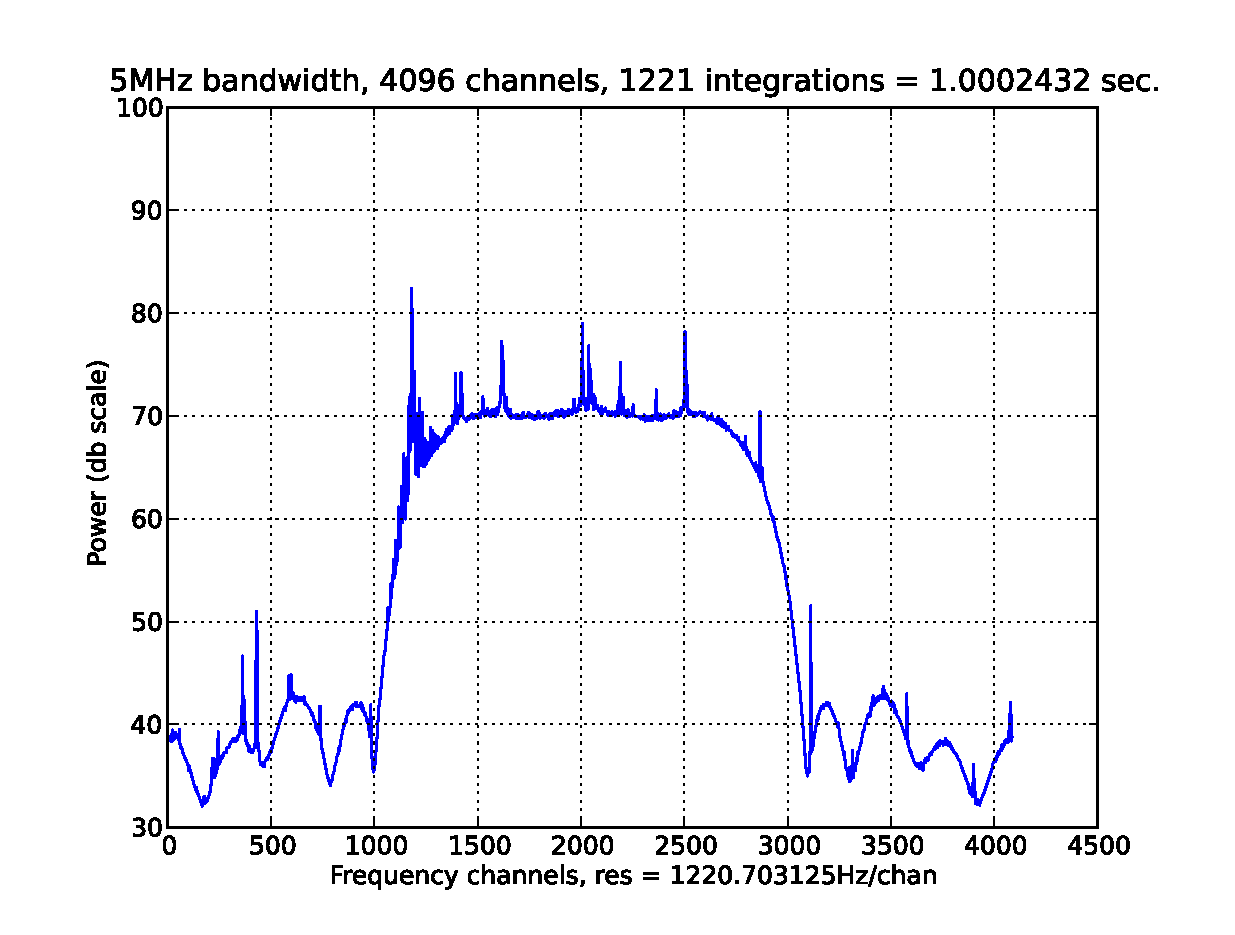
\includegraphics[width=1\linewidth]{5_4096_1221}
	\end{center}
	\caption{Visualizzazione di un segnale elaborato con il programma}
	\label{fig:correctness}
\end{figure}

Da questa immagine si capisce quindi che il programma elabora correttamente i
dati e produce una trasformazione corretta dei segnali.

\subsection{Riduzione del rumore}
Verifichiamo anche il corretto funzionamento del metodo delle somme dello stesso
segnale per attutire il rumore: nella figura \ref{fig:low_int} si vede un
segnale con 5 Mhz di banda ed elaborato a 512 canali, senza effettuare alcuna
somma di altre elaborazioni. Si pu\`o osservare con il grafico risultante sia
estremamente frastagliato e a malapena si riesce ad intuire la forma del rumore
introdotto dall'antenna, mentre gli eventuali segnali non sono nemmeno
distringuibili dal rumore di fondo.
\begin{figure}[htb]
	\begin{center}
		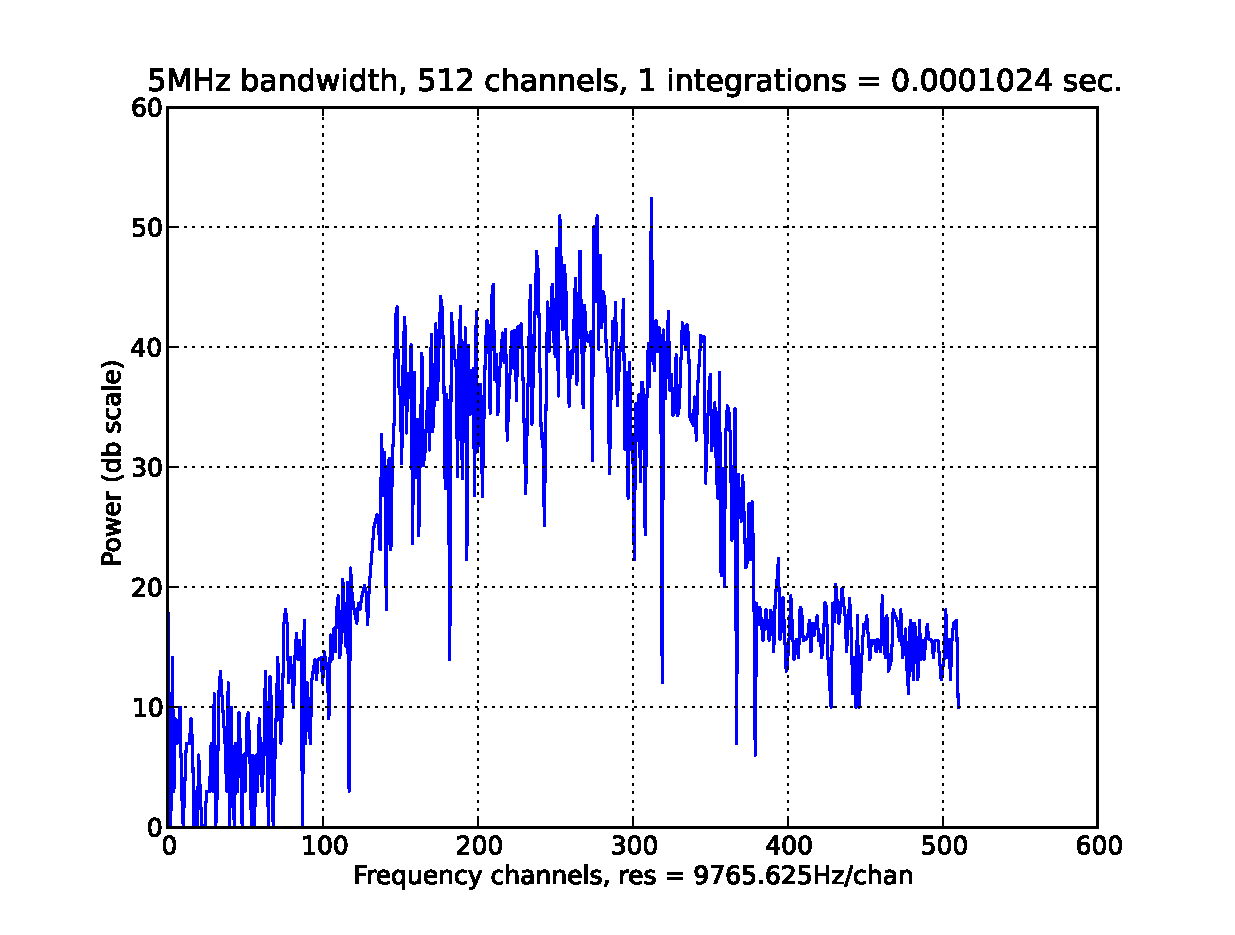
\includegraphics[width=1\linewidth]{5_512_1}
	\end{center}
	\caption{Segnale senza nessuna integrazione}
	\label{fig:low_int}
\end{figure}

Confrontiamo questa immagine con la figura \ref{fig:high_int} dove vengono
effettuate 97656 elaborazioni successive di un segnale nel tempo e poi sommate
tra di loro: in questa seconda immagine \`e perfettamente delineata la forma del
rumore dell'antenna cos\`i come sono perfettamente visibili i segnali presenti.
Si intuisce anche come le due immagini rappresentino la stessa cosa, anche se la
prima \`e un po' ``sfuocata'', non sufficientemente dettagliata, mentre la
seconda \`e molto pi\`u netta.
\begin{figure}[htb]
	\begin{center}
		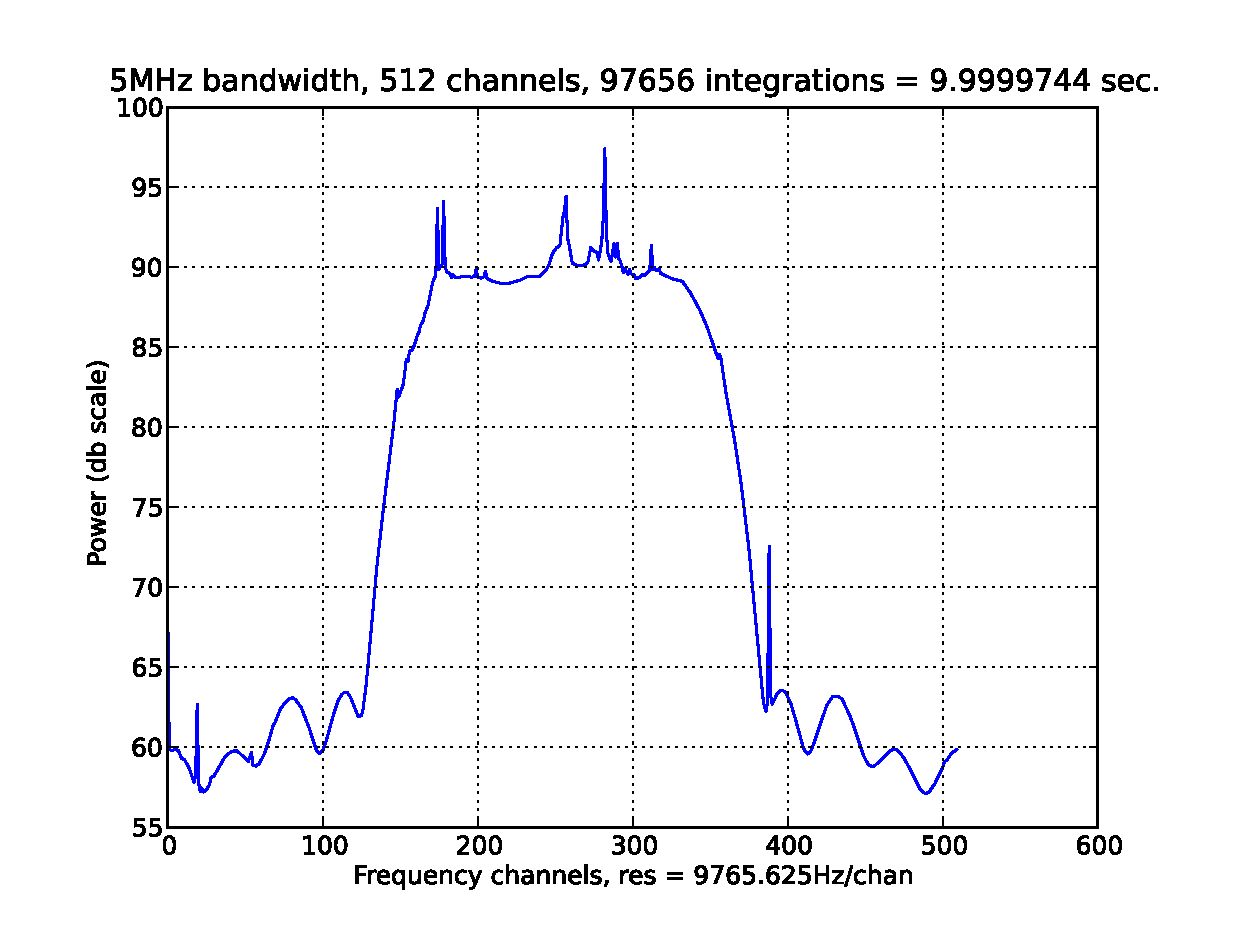
\includegraphics[width=1\linewidth]{5_512_97656}
	\end{center}
	\caption{Segnale con un elevato numero di integrazioni}
	\label{fig:high_int}
\end{figure}

Tuttavia va considerato anche che aumentando il numero di somme, aumenta anche
il tempo di elaborazione necessario: nel primo caso per calcolare i dati
rappresentati nell'immagine \`e stato richiesto un tempo di $0,00002$ secondi,
mentre nel secondo caso sono stati impiegati $2,7$ secondi.  Chiaramente va
ricercato un compromesso tra riduzione del rumore e tempo di calcolo,
compromesso che varia a seconda del tipo di analisi che si desidera fare: per
alcuni tipi di osservazioni va bene anche un segnale non molto ben definito,
purch\'e sia calcolato molto in fretta; per altri tipi di osservazioni, il
segnale deve essere definito molto precisamente, al costo di un maggiore tempo
di calcolo.

\subsection{Variazione del numero di canali}
Il numero di canali usati nel calcolo della \ac{FFT} influiscono risoluzione di
ognuno di questi canali: se i canali sono pochi, ogni canale rappresenta una
banda di frequenza piuttosto ampia, mentre con molti canali la banda di
frequenza si restringe. Aumentare il numero di canali permette di analizzare un
segnale pi\`u nel dettaglio, osservando anche variazioni tra frequenze molto
vicine tra loro. Al contrario, con pochi canali le frequenze vicine tra loro
vengono mediate. Per verificare questo fenomeno, si confrontino la figura
\ref{fig:low_chans} con la figura \ref{fig:high_chans}: nella seconda figura
tutta la zona colorata di blu \`e composta da oscillazioni vicinissime tra loro,
presenti anche nella prima figura, ma abbastanza distanziate da essere ben
visibili. Nella prima figura, ogni canale ha una risoluzione di $19531,25
Hz/canale$, mentre nella seconda ogni canale ha una risoluzione di $1,192
Hz/canale$.
\begin{figure}[htb]
	\begin{center}
		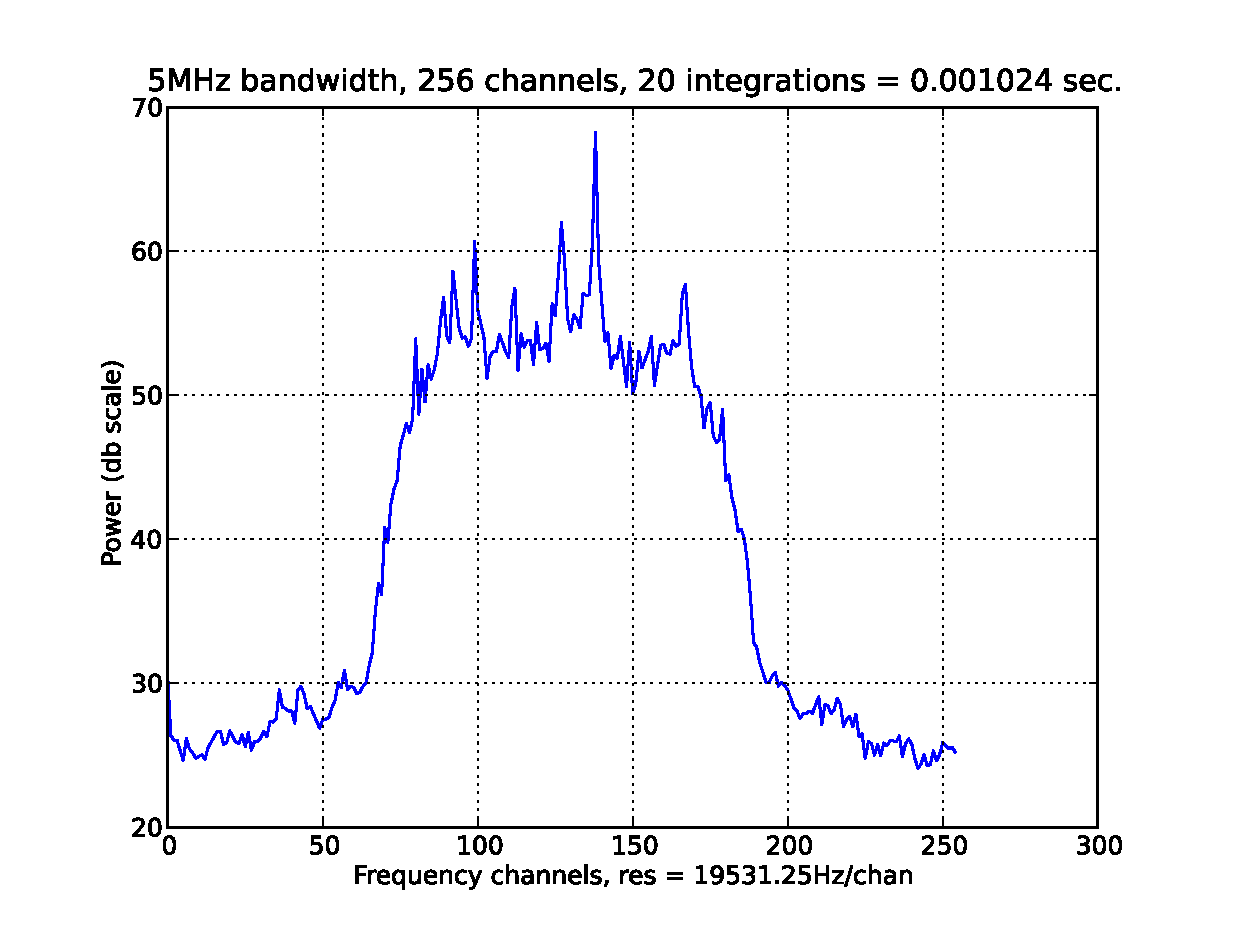
\includegraphics[width=1\linewidth]{5_256_20}
	\end{center}
	\caption{Segnale analizzato con pochi canali}
	\label{fig:low_chans}
\end{figure}

\begin{figure}[htb]
	\begin{center}
		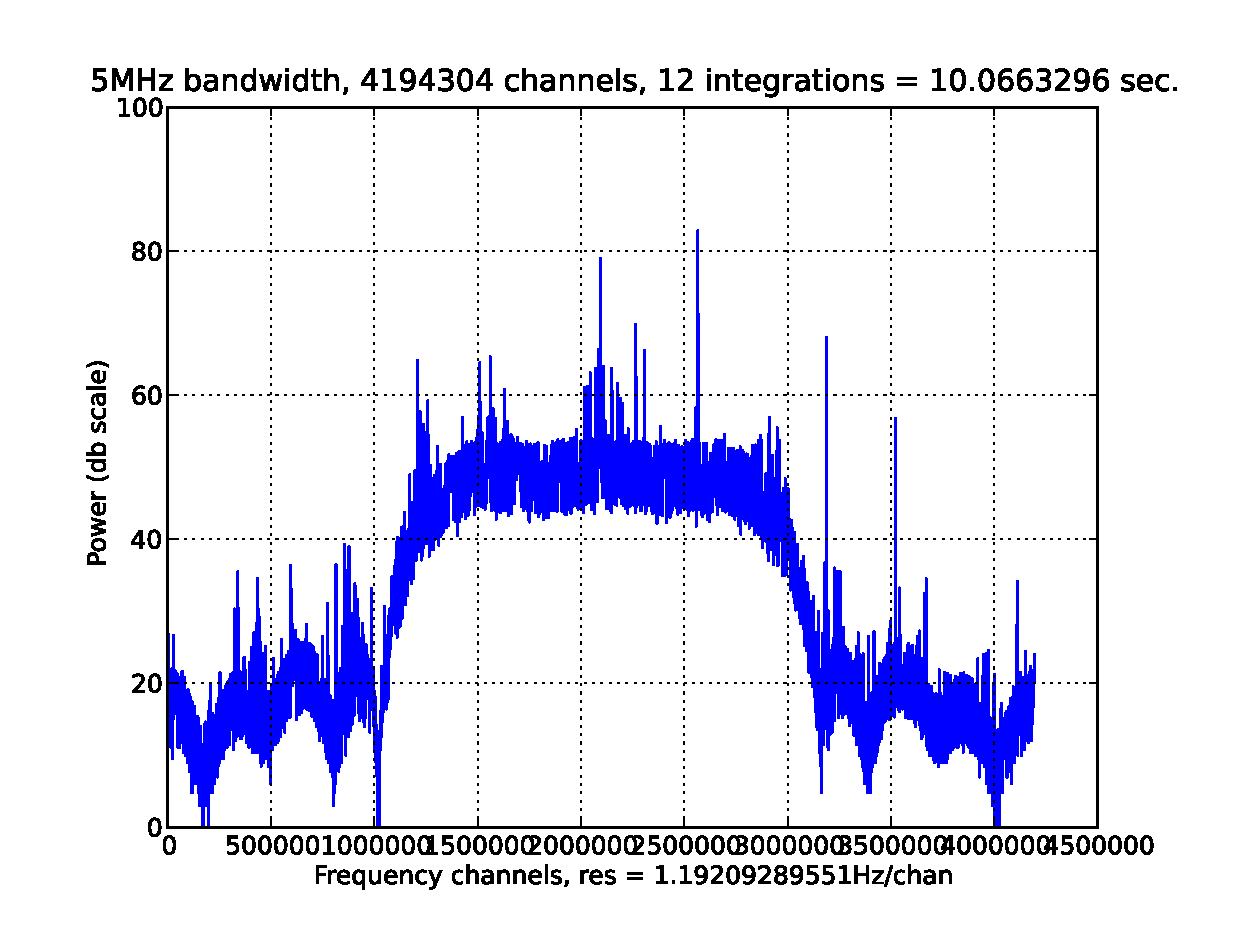
\includegraphics[width=1\linewidth]{5_4194304_12}
	\end{center}
	\caption{Segnale analizzato con molti canali}
	\label{fig:high_chans}
\end{figure}

Come per la riduzione del rumore di fondo, aumentando il numero di canali
aumenta il tempo di calcolo; allo stesso modo il compromesso tra numero di
canali e tempo di calcolo dipende dal tipo di analisi che si intende effettuare.

\section{Verifica delle prestazioni}
\ctable[
    cap=Alcuni tempi di calcolo,
    caption=Esempio di alcuni tempi di calcolo,
    label=tab:tests
]{llllll}{
\tnote[a]{Tempo espresso in secondi}
\tnote[b]{Dimensione dei files in bytes}
\tnote[c]{Si intende il tempo impiegato per effettuare tutte le \ac{FFT} e le somme dei risultati.}
}{
                \FL
Can. & Integr. & Tempo totale\tmark[a] & Dim. output\tmark[b] & Segnali output & Tempo trasf.\tmark[a]\tmark[c] \ML
256 & 1 & 4.831 & 96423936 & 94164 & 5.13041e-05\NN
256 & 20 & 5.984 & 5974016 & 5834 & 0.00102571\NN
256 & 195 & 3.952 & 403456 & 394 & 0.0100305\NN
256 & 195313 & 24.182 & 2048 & 2 & 12.091\NN
512 & 1 & 5.087 & 101545984 & 49583 & 0.000102596\NN
512 & 98 & 9.040 & 1841152 & 899 & 0.0100556\NN
65536 & 1 & 5.115 & 101974016 & 389 & 0.0131491\NN
65536 & 76 & 6.267 & 1572864 & 6 & 1.0445\NN
524288 & 1 & 3.962 & 77594624 & 37 & 0.107081\NN
524288 & 95 & 38.645 & 6291456 & 3 & 12.8817\NN
4194304 & 1 & 6.242 & 100663296 & 6 & 1.04033\NN
4194304 & 12 & 38.022 & 50331648 & 3 & 12.674\LL
}

Una volta determinato che il programma funziona, \`e stabile e produce dei
risultati corretti, si pu\`o verificare il livello di prestazioni. Per questo
sono stati fatti dei test dove si aumentava man mano il numero di canali e il
numero di integrazioni. L'aumento del numero di integrazioni \`e stato studiato
in modo che l'ordine di grandezza del tempo di calcolo previsto aumentasse ad
ogni test: se si osserva le prime righe della tabella \ref{tab:tests} si nota
che all'aumentare del numero di integrazioni il tempo si moltiplica all'incirca
per 10.\footnote{Notare che nella prima riga si impiega 20 volte meno tempo
    rispetto alla seconda. Questo perch\'e le integrazioni avrebbero dovuto
    essere 2 per ottenere un tempo 10 volte inferiore.}
Per valutare il numero di integrazioni necessarie, la formula utilizzata \`e
$integrations = \frac{bandwidth}{channels} * time$. Considerando che tutti i
segnali utilizzati hanno 5 Mhz di banda, \`e facile ricavare il numero di
integrazioni richieste. I tempi testati oscillano tra $10^-3$ e $10$.
I canali aumentano raddoppiando, per motivi visti nel paragrafo
\ref{analisi_sintesi}, e ogni volta che si incrementa il numero di canali,
conseguentemente incrementa il tempo di calcolo.

L'obiettivo di questi test \`e di verificare un eventuale limite superiore del
programma nel calcolare le trasformate. Avendo predeterminato i tempi di calcolo
desiderati, \`e facile verificare la tenuta dell'algoritmo: si osservino le
tabelle nell'appendice \ref{test_tables}, si noter\`a che tutti i tempi
rientrano nelle previsioni.

\chapter{Conclusioni e sviluppi futuri}
\label{conclusions}
\section{Sviluppi futuri}
\subsection{Librerie alternative}
\label{altlib}
\subsection{\ac{seti}}
\label{seti}
Implementazione acquisizione.


\bibliographystyle{alpha}
\bibliography{thesis}
\end{document}
